%\documentclass[dvipdfmx,a4paper,12pt]{amsart}
\documentclass[dvipdfmx,a4paper,12pt]{article} %titleとe-mailをコメントアウトする.


%%% Packages %%%
\setlength{\lineskip}{0pt}

% --- 和文フォント設定 (ゴシックを使うなら) ---amsartを使う時はコメントアウト
\renewcommand{\kanjifamilydefault}{\gtdefault}
\usepackage{otf}          % min10を避けるため
\usepackage{pxrubrica}    % 和文ルビ

% --- 基本パッケージ ---
\usepackage{graphicx}
\usepackage[all]{xy}
\usepackage{wrapfig}
\usepackage{pgfplots}
\usepackage{color}
\usepackage[dvipsnames]{xcolor}

% --- 数学関連 ---
\usepackage{amsmath,amssymb,amsthm,amsfonts,mathtools}
\usepackage{amscd,dsfont,bigdelim,braket,physics,mathrsfs,bm}

% --- 書式・リスト関連 ---
\usepackage{latexsym}
\usepackage{setspace}
\usepackage{multirow}
\usepackage{enumerate}
\usepackage{enumitem}

% --- コメント・取消線など ---
\usepackage{comment}
\usepackage[normalem]{ulem} % \emph の下線化を抑止(cancelと共存)

% --- URL・文字コード ---
\usepackage{url}
% \usepackage[utf8]{inputenc}  % ← 使用しているエンジンがuplatexなら不要、pdflatexなら有効に

% --- showkeys(常に表示) ---
\usepackage{showkeys}
\renewcommand*{\showkeyslabelformat}[1]{%
  \fbox{\parbox{1.6cm}{\normalfont\tiny\sffamily#1\vspace{6mm}}}%
}
% --- hyperrefは最後に読み込む ---
\usepackage[dvipdfmx,colorlinks,linkcolor=blue,anchorcolor=blue,citecolor=blue]{hyperref}

%%% レイアウト調整 %%%
%%% レイアウト調整(geometryに統一) %%%
\usepackage[
  top=20mm,        % 上余白
  bottom=20mm,     % 下余白
  left=25mm,       % 左余白
  right=25mm,      % 右余白
  headheight=12pt, % ヘッダー高さ(必要なら)
  headsep=10mm,    % ヘッダーと本文の間
  footskip=32pt,   % 本文とフッターの距離
  includehead,     % ヘッダー分も高さに含める
  includefoot      % フッター分も高さに含める
]{geometry}

%%% 行間調整(適宜 1.2 などに変更) %%%
\usepackage{setspace}
\setstretch{1.1}

% --- 段落設定 --- 文字の行間ならここを変更する
\setlength{\parskip}{5pt}   % 段落間のスペース
\setlength{\parindent}{0pt}   % 段落先頭の字下げをなくす


%%% 追加(重複なし)パッケージ・設定 %%%

% --- 目次の体裁調整 ---
\usepackage{tocloft}
%\renewcommand{\contentsname}{目次} % 日本語化
\setlength{\cftbeforesecskip}{0pt}
\setlength{\cftbeforesubsecskip}{0pt}
\setlength{\cftbeforesubsubsecskip}{0pt}

% --- セクション見出しの体裁調整 ---
%\usepackage{titlesec}
%\titleformat*{\section}{\Large\bfseries}
%\titleformat*{\subsection}{\large\bfseries}
%\titlespacing*{\section}{0pt}{1.5ex plus .2ex minus .2ex}{0.8ex plus .1ex}
%\titlespacing*{\subsection}{0pt}{1.0ex plus .2ex minus .2ex}{0.5ex plus .1ex}

% --- ヘッダー/フッター設定 ---
%\usepackage{fancyhdr}
%\pagestyle{fancy}
%\fancyhf{}
%\rhead{岩井 雅崇}
%\lhead{大阪大学 数学専攻}
%\cfoot{\thepage}

% -- enumerate, itemize行間設定
\usepackage{enumitem} % デフォルト設定
\setlist[itemize]{itemsep=3pt, parsep=0pt}
\setlist[enumerate]{itemsep=3pt, parsep=0pt}
% "変更する際は右を使う" \setlength{\parskip}{0cm} % 段落間\setlength{\itemsep}{5pt} % 項目間

% --- tcolorbox 設定 ---%\begin{tcolorbox}[mybox]と使う
\usepackage[most]{tcolorbox}
\tcbuselibrary{breakable, skins, theorems}
\tcbset{
  mybox/.style={
    colback = white,
    colframe = green!35!black,
    fonttitle = \bfseries,
    breakable = true
  }
}

%--緑枠自動化
\AtBeginEnvironment{prop}{\begin{tcolorbox}[mybox]}
\AtEndEnvironment{prop}{\end{tcolorbox}}
\AtBeginEnvironment{lem}{\begin{tcolorbox}[mybox]}
\AtEndEnvironment{lem}{\end{tcolorbox}}
\AtBeginEnvironment{thm}{\begin{tcolorbox}[mybox]}
\AtEndEnvironment{thm}{\end{tcolorbox}}
\AtBeginEnvironment{defn}{\begin{tcolorbox}[mybox]}
\AtEndEnvironment{defn}{\end{tcolorbox}}
\AtBeginEnvironment{cor}{\begin{tcolorbox}[mybox]}
\AtEndEnvironment{cor}{\end{tcolorbox}}
\AtBeginEnvironment{ques}{\begin{tcolorbox}[mybox]}
\AtEndEnvironment{ques}{\end{tcolorbox}}
\AtBeginEnvironment{conj}{\begin{tcolorbox}[mybox]}
\AtEndEnvironment{conj}{\end{tcolorbox}}


% --- TikZ 設定 ---
\usepackage{tikz}
\usetikzlibrary{positioning, arrows.meta, fit, calc, backgrounds}
\pgfdeclarelayer{background}
\pgfdeclarelayer{foreground}
\pgfsetlayers{background,main,foreground}

% --- footnote がページをまたがない設定 ---
\interfootnotelinepenalty=10000

% --- 目次に表示する階層の深さ ---
\setcounter{tocdepth}{2}

% --- 日本語目次---
\usepackage{pxjahyper}

%--newtheorem%--newcommand----

\newtheorem{thm}{Theorem}[section] 
\newtheorem{theo}[thm]{Theorem}
\newtheorem{cor}[thm]{Corollary}
\newtheorem{prop}[thm]{Proposition}
\newtheorem{conj}[thm]{Conjecture}
\newtheorem*{mainthm}{Theorem}
\newtheorem{deflem}[thm]{Definition-Lemma}
\newtheorem{lem}[thm]{Lemma}
\theoremstyle{definition} 
\newtheorem{defn}[thm]{Definition}
\newtheorem{propdefn}[thm]{Proposition-Definition} 
\newtheorem{lemdefn}[thm]{Lemma-Definition} 
\newtheorem{thmdefn}[thm]{Theorem-Definition} 
\newtheorem{eg}[thm]{Example} 
\newtheorem{ex}[thm]{Example} 
\newtheorem{ques}[thm]{Question}
\newtheorem{remin}[thm]{Reminder}
\theoremstyle{remark}
\newtheorem{rem}[thm]{Remark}
\newtheorem{setup}[thm]{Setup}
\newtheorem{obs}[thm]{Observation}
\newtheorem{notation}[thm]{Notation}
\newtheorem{cl}{Claim}
\newtheorem{claim}[thm]{Claim}
\newtheorem{assup}[thm]{Assumption}
\newtheorem{step}{Step}
\newtheorem*{clproof}{Proof of Claim}
\newtheorem{cln}[thm]{Claim}
\newtheorem*{ack}{Acknowledgements} 
\numberwithin{equation}{section}
\newtheorem{case}{Case}



\newcommand{\rk}[0]{\operatorname{rk}}
\newcommand{\supp}[0]{\operatorname{Supp}}
\newcommand{\Rad}[0]{\operatorname{Rad}}
\newcommand{\Sha}[0]{\operatorname{Sha}}
\newcommand{\sha}[0]{\operatorname{sha}}
\newcommand{\eend}[0]{\operatorname{End}}
\newcommand{\codim}[0]{\operatorname{codim}}
\newcommand{\nd}[0]{\operatorname{nd}}
\renewcommand{\rank}[0]{\operatorname{rank}}
\newcommand{\degree}[0]{\operatorname{deg}}
\newcommand{\Exc}[0]{\operatorname{Exc}}
\newcommand{\pr}{{\rm pr}}
\newcommand{\id}{{\rm id}}
\newcommand{\Sym}{{\rm Sym}}
\newcommand{\End}[0]{\operatorname{End}}
\newcommand{\Coker}[0]{\operatorname{Coker}}

\newcommand{\Supp}{{\rm Supp}}
\newcommand{\Hom}[0]{\mathscr{H}\!\textit{om}}
\newcommand{\Ext}[0]{\mathscr{E}\!\textit{xt}}
\newcommand{\GL}[0]{\operatorname{GL}}
\newcommand{\SheafHom[1]}{\mathscr{H}\!\!\!\text{\calligra om}_{\,{#1}}}
\newcommand{\PGL}[0]{\mathbb{P}\GL(r,\C)}

\newcommand{\Alb}{{\rm Alb}}
\newcommand{\verti}{{\rm vert}}
\newcommand{\hor}{{\rm hor}}
\newcommand{\univ}{{\rm univ}}
\newcommand{\Tor}{{\rm tor}}
\newcommand{\shaf}{\mathrm{sha}}
\newcommand{\Shaf}{\mathrm{Sha}}
\newcommand{\reg}{{\rm{reg}}}
\newcommand{\sing}{{\rm{sing}}}
\newcommand{\qt}{{\rm{qt}}}
\newcommand\sO{{\mathcal O}}
\newcommand{\Div}[0]{\operatorname{div}}
\newcommand{\ddbar}{dd^c}
\newcommand{\cV}{\mathcal{V}}
\newcommand{\deldel}{\sqrt{-1}\partial \overline{\partial}}
\newcommand{\dbar}{\overline{\partial}}
\newcommand{\I}[1]{\mathcal{I}(#1)}
\newcommand{\Aut}[1]{\mathrm{Aut}(#1)}
\newcommand{\Ker}[1]{\mathrm{Ker}(#1)}
\newcommand{\Image}[1]{\mathrm{Im}(#1)}
\DeclareMathOperator{\Ric}{Ric}
\DeclareMathOperator{\Vol}{Vol}
 \newcommand{\pdrv}[2]{\frac{\partial #1}{\partial #2}}
 \newcommand{\drv}[2]{\frac{d #1}{d#2}}
  \newcommand{\ppdrv}[3]{\frac{\partial #1}{\partial #2 \partial #3}}
\newcommand{\underalign}[2]{\quad \underset{\mathclap{\strut #1}}{#2}\quad}
\newcommand{\polar}{\beta}
  
\newcommand{\R}{\mathbb{R}}
\newcommand{\Z}{\mathbb{Z}}
\newcommand{\N}{\mathbb{Z}_+}
\newcommand{\C}{\mathbb{C}}
\newcommand{\Q}{\mathbb{Q}}
\newcommand{\D}{\mathbb{D}}
\newcommand{\mP}{\mathbb{P}}
\newcommand{\mO}{\mathcal{O}}
\newcommand{\B}{\mathds{B}}
\newcommand{\tl}{\hspace{-0.8ex}<\hspace{-0.8ex}}
\renewcommand{\tr}{\hspace{-0.8ex}>}

\newcommand{\xb}[1]{\textcolor{blue}{#1}}
\newcommand{\xr}[1]{\textcolor{red}{#1}}
\newcommand{\xm}[1]{\textcolor{magenta}{#1}}



\title{学祭でのパズル}
\author{岩井雅崇 (大阪大学)}
%\address{Department of Mathematics, Graduate School of Science, Osaka City University 3-3-138, Sugimoto, Sumiyoshi-ku Osaka, 558-8585Japan} 
%\email{{\tt masataka.math@gmail.com}}
%\email{{\tt masataka.math@gmail.com, masataka@sci.osaka-cu.ac.jp}}



\date{\today, version 0.01}


\renewcommand{\thefootnote}{\arabic{footnote}}

\baselineskip = 15pt
\footskip = 32pt

\begin{document}

\maketitle 

展示用のパズルをまとめたものです. 
\footnote{メールアドレス {\tt masataka.math@gmail.com, masataka@sci.osaka-cu.ac.jp}}

\section{タイル1. }
図1のようなチェス盤は, 図2のような2×1のタイルで埋め尽くすことができないことを示せ.

ただし2×1のタイルは重なり合ってはいけないしはみ出てはいけない.
\begin{figure}[htbp]
\begin{center}
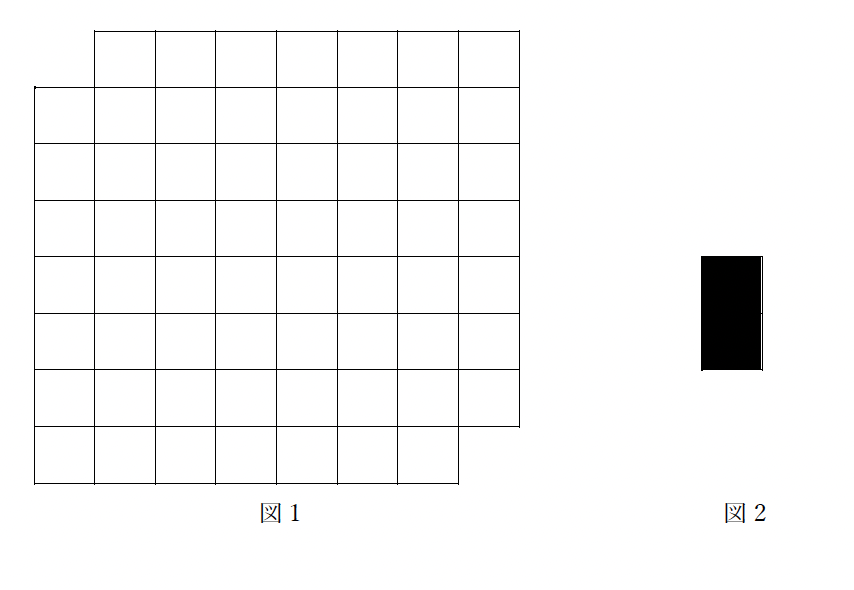
\includegraphics[width=80mm]{tile1.png}
\end{center}
\end{figure}


\section{タイル2. }
図1のような8×8のタイルの上に, 1×1タイルを好きなところにおく. 
このとき1×1タイルをどこにおいても, 図2のようなのタイルで埋め尽くすことができることを示せ.

ただし図2のようなタイルは重なり合ってはいけないしはみ出てはいけない.
\begin{figure}[htbp]
\begin{center}
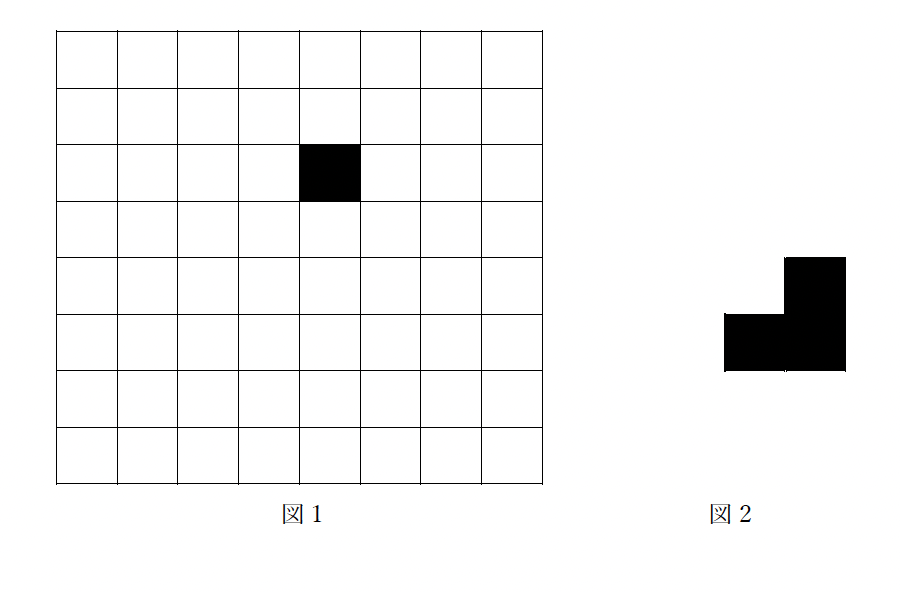
\includegraphics[width=80mm]{tile2.png}
\end{center}
\end{figure}

\section{タイル3. }
大きなタイルをたくさんの(有限個の)小さな長方形に分割した. 
その際全ての小さな長方形の縦の長さもしくは横の長さのどちらか(あるいは両方ともが)整数であった.

\vspace{5pt}
このとき, 大きな長方形の縦の長さもしくは横の長さのどちらか(あるいは両方とも)整数であることを示せ.
\begin{figure}[htbp]
\begin{center}
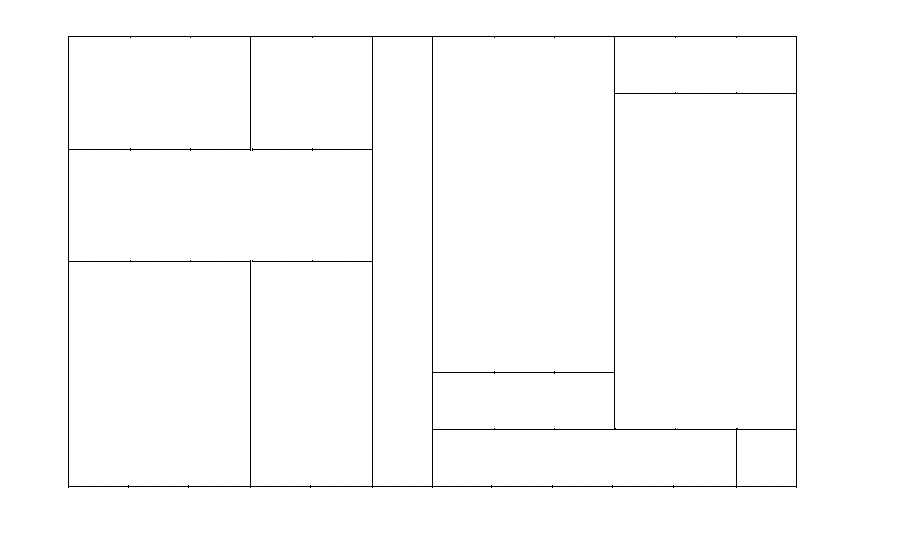
\includegraphics[width=80mm]{tile3.png}
\end{center}
\end{figure}





\section{Kontsevichのパズル}
図1のようにタイルが無限に並んでいて, 左下のみ黒で他は白であるものを考える.
次の操作を何回やっても, 図2の赤色の部分に黒のタイルがあることを示せ. 

\vspace{5pt}
[操作] 図1のように上も右も白であるような黒のタイルを選び, それを白タイルに変えて, その上も右も黒のタイルに変える.

\begin{figure}[htbp]
\begin{center}
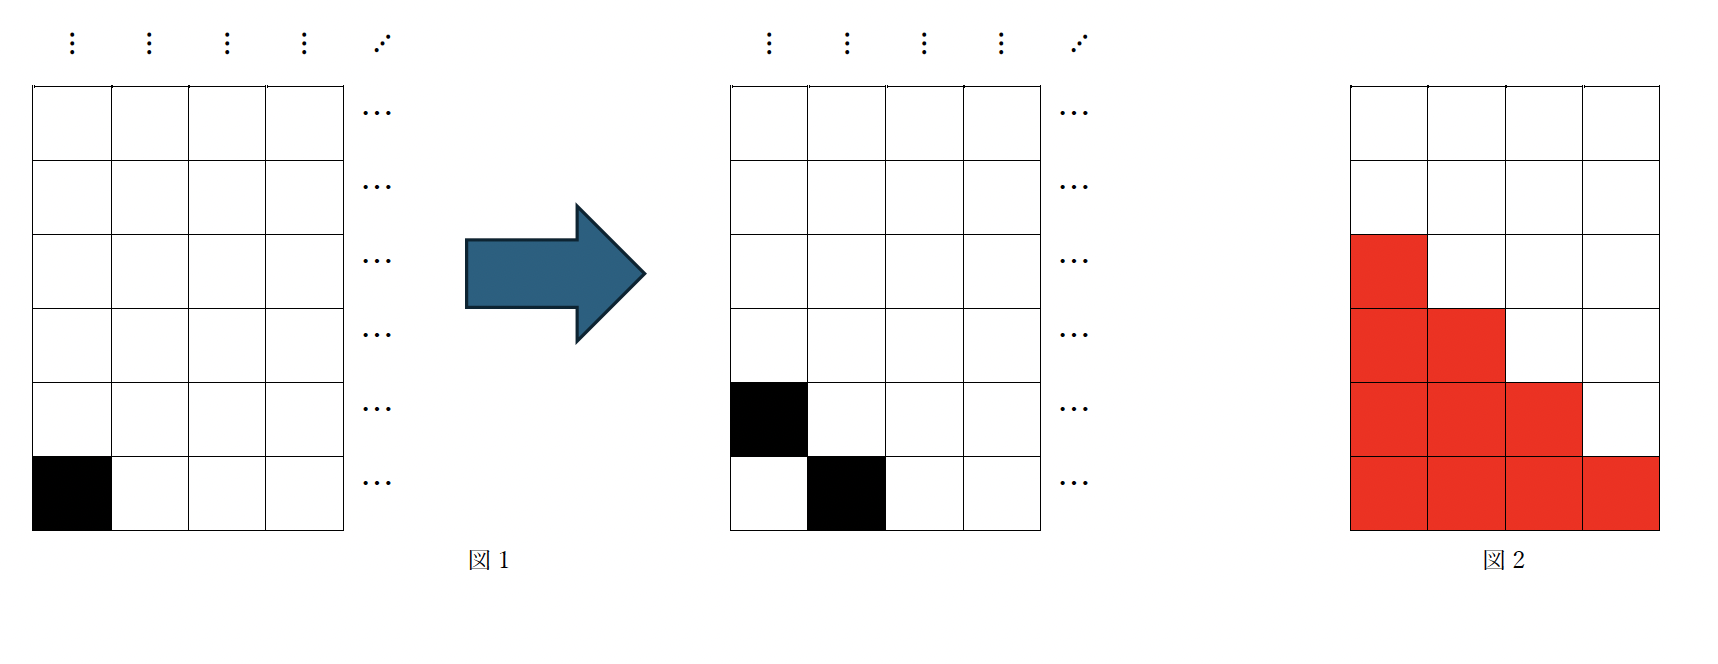
\includegraphics[width=100mm]{kont.png}
\end{center}
\end{figure}


\section{ドブル}
7色(赤, 橙, 黄, 緑, 青, 藍, 紫) のペンと7枚のカードある. 次のルールを考える.
\begin{enumerate}
    \setlength{\parskip}{0cm} 
  \setlength{\itemsep}{0cm} 
\item どのカードにも相異なる3 色の$\bullet$印がある.
\item どの2 枚のカードを取っても, 1 つだけ共通する色の$\bullet$印がある.
\end{enumerate}
上のルール2 つを満たすように色ペンを使ってカードに$\bullet$印を書くことはできるだろうか?

[補足] これをゲームにしたのがドブルである. ドブルで使うカードには, どんな2枚のカードを取っても共通する絵柄が必ず一つのみある. 

\section{11111.....}
$p$を2や5でない素数とする. 
$11111\cdots 111$という1が何個か並んだ形の$p$の倍数が存在することを示せ.

\vspace{10pt}
例えば...
\begin{itemize}
    \setlength{\parskip}{0cm} 
  \setlength{\itemsep}{0cm} 
  \item $p=3$の場合は111は3の倍数.
  \item $p=7$の場合は111111は7の倍数.
  \item $p=11$の場合は11は11の倍数.
  \end{itemize}
  
\section{2010年大阪大学理系第3問}
$l,m,n$を3以上の整数とする. 等式
$$
\left( \frac{n}{m} - \frac{n}{2} + 1 \right)l = 2
$$
を満たす$l,m,n$の組を全て求めよ. 

[補足] 実はこの方程式は隣の部屋の展示物と大きな関連がある. 



\section{コイン 1}
テーブル上に10個の硬貨が一列に並んでいる. 
その硬貨の額は1円か5円か10円である. 

あなたと私の二人で次のルールの下, 以下のゲームを行う.
\begin{itemize}
\item 列のうち左端か右端の硬貨を取る. その後次の人に手番をわたす.
\item とった硬貨の総額が多い方が勝ち. 同じであれば引き分け. 
\end{itemize}

ゲームに"負けたくない"あなたなら先手・後手どちらを選べば良いだろうか?
またその際どのような戦略を取れば良いだろうか?

\begin{figure}[htbp]
\begin{center}
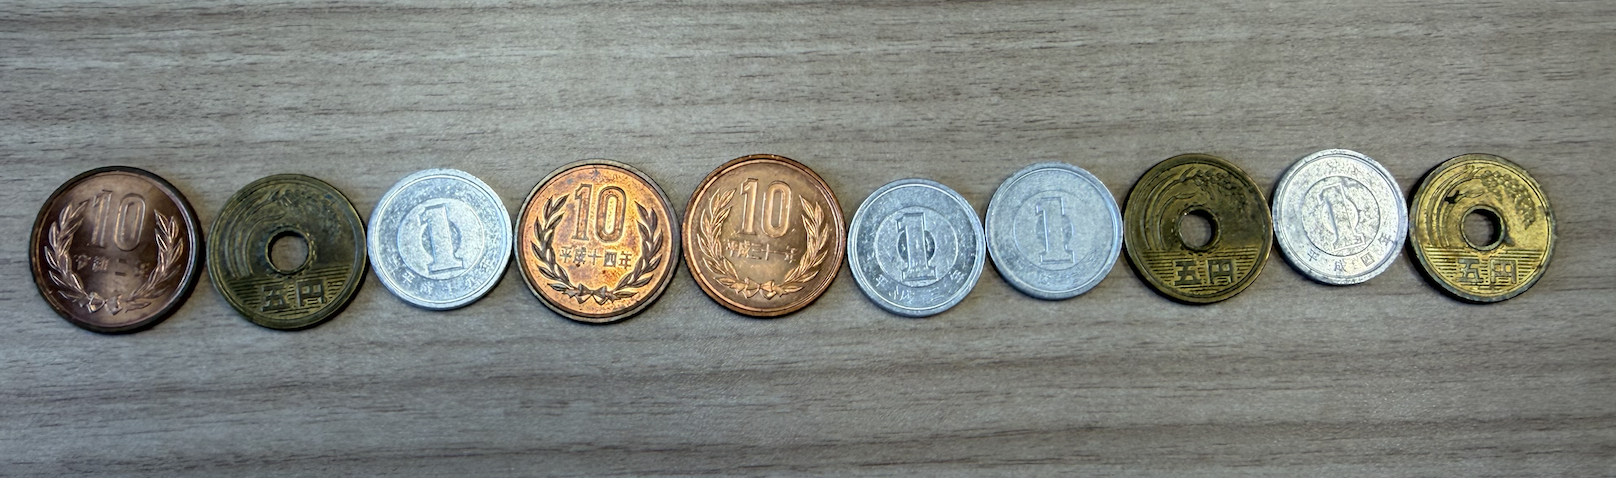
\includegraphics[width=80mm]{coin1.png}
\end{center}
\end{figure}

\section{コイン 2}
テーブル上に25個の1円玉がある.
あなたと私の二人で次のルールの下, 以下のゲームを行う.

\begin{itemize}
\item テーブルの上の1円玉から, 1枚か2枚か3枚のコインを取る. その後次の人に手番をわたす.
\item 最後の1円玉を取った人が負け.
\end{itemize}

ゲームに"負けたくない"あなたなら先手・後手どちらを選べば良いだろうか?
またその際どのような戦略を取れば良いだろうか?

\begin{figure}[htbp]
\begin{center}
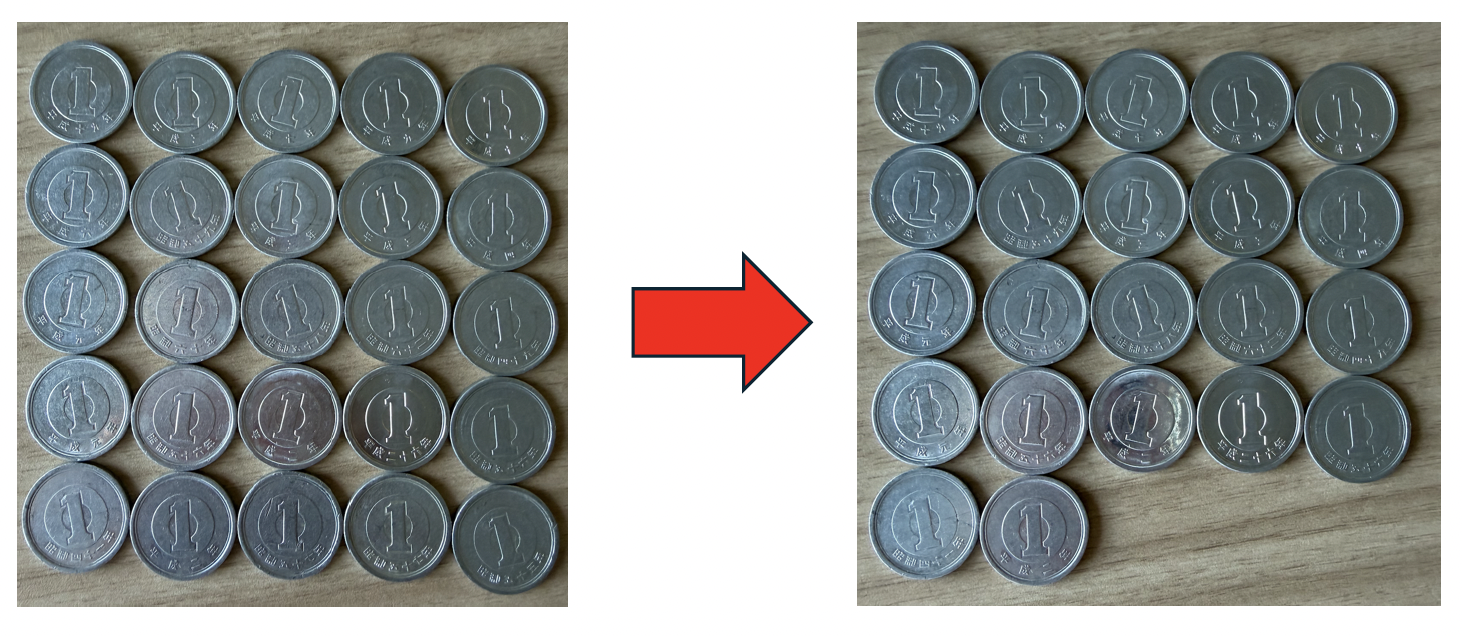
\includegraphics[width=80mm]{coin2.png}
\end{center}
\end{figure}

\section{コイン 2'}
テーブル上に25個の1円玉がある.
あなたと私の二人で次のルールの下, 以下のゲームを行う.

\begin{itemize}
\item テーブルの上の1円玉から, \underline{1枚か3枚か4枚}のコインを取る. その後次の人に手番をわたす.
\item 最後の1円玉を取った人が負け.
\end{itemize}


ゲームに"負けたくない"あなたなら先手・後手どちらを選べば良いだろうか?
またその際どのような戦略を取れば良いだろうか?

\section{コイン 3}
1円玉が裏向きに$5 \times 5$の正方形に並んでいる.
次の操作を考える. 
\begin{itemize}
\item 縦か横に連続する3枚の1円玉を同時にひっくり返す.
\end{itemize}

 この操作を何回かして全ての1円玉を表向きにできるか?
 
 \begin{figure}[htbp]
\begin{center}
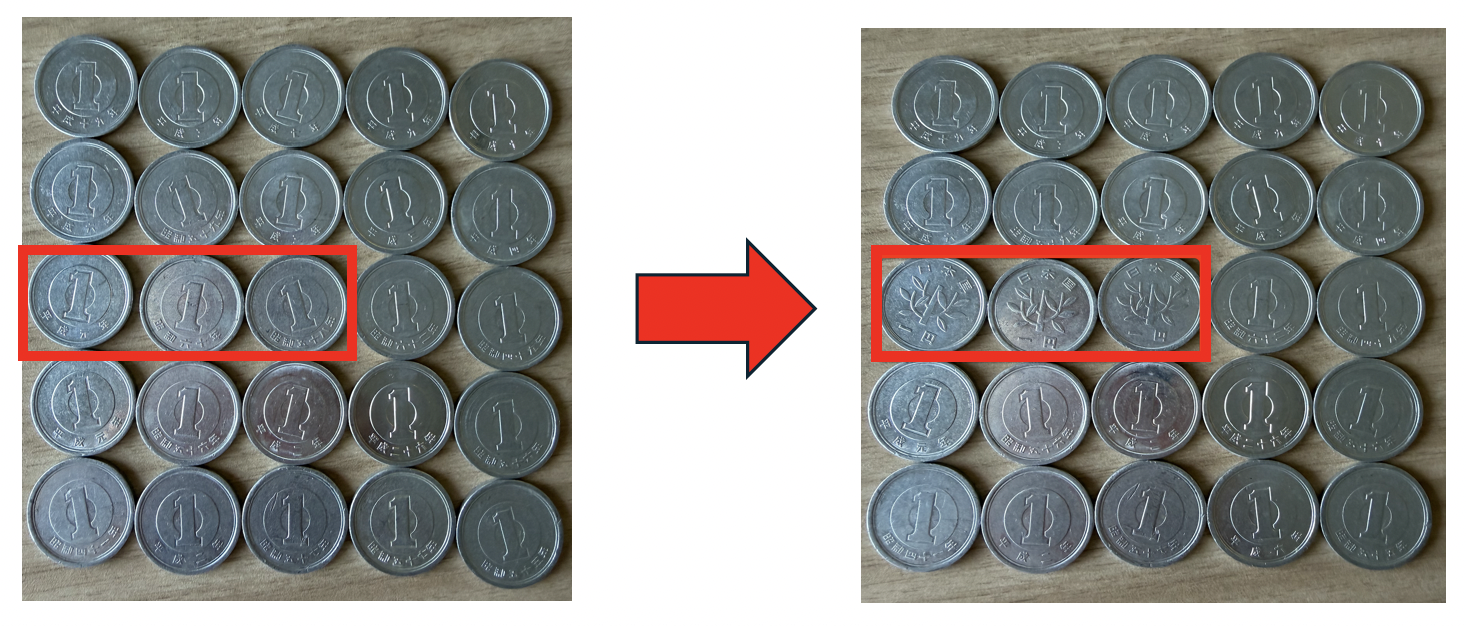
\includegraphics[width=80mm]{coin3.png}
\end{center}
\end{figure}

\section{$1 + \sqrt{2}$}
$(1 + \sqrt{2})^{2025}$の小数第100位を求めよ.





 \end{document}
